\chapter{Digital Image Processing}
\label{ch:imageproc}

\begin{objectives}
\begin{itemize}
  \item Treat an image as a sampled function, and filter it by convolution.
  \item Smooth images with Gaussian kernels, and understand separability and cost.
  \item Compute image gradients robustly with derivative-of-smoothing kernels such as Sobel and Scharr.
  \item Understand why images must be blurred before they are down-sampled, and build Gaussian pyramids.
  \item Interpolate images at sub-pixel positions, find local maxima, and refine them to sub-pixel accuracy.
  \item Know how photometric changes affect intensity-based methods.
\end{itemize}
\end{objectives}

Feature detection and tracking (\cref{ch:frontend}) operate on raw pixel arrays: they smooth them, differentiate them, shrink them and sample them between
pixels. This chapter develops these operations from first principles, as far as the front end needs them.

% ==============================================================================
\section{Images as functions}

A grayscale image is a function $I(u, v)$ giving the brightness at image position $(u, v)$, sampled on the integer grid of pixel centers and quantized,
typically to integers between 0 and 255. In memory it is a 2D array indexed by row and column, $I[\text{row}, \text{col}] = I(u = \text{col}, v = \text{row})$; mixing up the
two orders is a classic bug. Color images have three such channels; a monochrome image can be formed as a weighted sum of them. EuRoC's cameras are
monochrome.

Between pixels, $I$ is undefined until we decide how to interpolate it (\cref{sec:interpolation}). Its derivatives must be approximated by differences of
nearby pixels (\cref{sec:image-derivatives}). Both operations are sensitive to noise and to aliasing, which is what the rest of this chapter is about.

% ==============================================================================
\section{Linear filtering}

\subsection{Correlation and convolution}

\index{convolution}
\termi{Linear filtering}{linear filtering} replaces each pixel by a weighted sum of its neighbors, with the weights given by a small array $h$, the \emph{kernel}. Two closely related
forms exist:
\begin{equation}
\begin{aligned}
  \text{correlation:}&\quad (h\star I)[u, v] = \sum_{i,j}h[i, j]\,I[u + i, v + j], \\
  \text{convolution:}&\quad (h * I)[u, v] = \sum_{i,j}h[i, j]\,I[u - i, v - j] .
\end{aligned}
\end{equation}
Convolution flips the kernel; for symmetric kernels the two coincide. Both are \emph{linear} and \emph{shift-invariant}: filtering a shifted image gives the shifted
filtered image. Convolution is also commutative and associative, so a cascade of filters equals a single filter, $h_2 * (h_1 * I) = (h_2 * h_1) * I$. Near the image
border the kernel extends past the edge, and the missing pixels must be invented: by zeros, by replicating the border, or by reflecting the image. Results
within a kernel radius of the border are always less reliable, which is why detectors ignore a margin there.

A $k\times k$ kernel costs $k^2$ multiplications per pixel. A kernel that factors as an outer product of a column and a row, $h = h_vh_u\T$, is \emph{separable}: filtering
with $h$ equals filtering the rows with $h_u$ and then the columns with $h_v$, at a cost of $2k$ per pixel.

\subsection{Smoothing}

Averaging neighbors reduces noise. The simplest kernel, the \emph{box filter}, averages a $k\times k$ square. The \term{Gaussian filter} weights neighbors by
\begin{equation}
  G_\sigma(u, v) = \frac{1}{2\pi\sigma^2}\exp\!\Big(-\frac{u^2 + v^2}{2\sigma^2}\Big) = g_\sigma(u)\,g_\sigma(v), \qquad g_\sigma(x) = \frac{1}{\sqrt{2\pi}\sigma}e^{-x^2/2\sigma^2},
\end{equation}
sampled at integer offsets, truncated at about $\pm3\sigma$ and renormalized to sum to one. The factorization shows that it is separable. The Gaussian is preferred
over the box because it has no sharp edges: its frequency response is itself a Gaussian, which removes high frequencies smoothly without the ripples of the
box filter. Cascading two Gaussian filters gives a Gaussian whose variances add, $G_{\sigma_1}*G_{\sigma_2} = G_{\sqrt{\sigma_1^2 + \sigma_2^2}}$. Small Gaussians are well
approximated by binomial kernels, $\tfrac14[1, 2, 1]$ and $\tfrac1{16}[1, 4, 6, 4, 1]$ in each direction.

% ==============================================================================
\section{Image derivatives}
\label{sec:image-derivatives}

\index{image gradient}
The \term{image gradient} $\nabla I = (I_u, I_v)$ points in the direction of fastest brightness increase, and its magnitude measures the local contrast. It is
approximated by differences, for example the central difference $I_u[u, v] \approx \tfrac12(I[u + 1, v] - I[u - 1, v])$, a correlation with $\tfrac12[-1, 0, 1]$.

Differentiation amplifies noise: a derivative multiplies each frequency component by its frequency, so pixel-to-pixel noise, the highest frequency present,
is amplified most. The remedy is to smooth before differentiating, and since both are convolutions, to combine them into one kernel. The \emph{Sobel}
operator smooths across the derivative direction with $[1, 2, 1]$ and differentiates along it:
\begin{equation}
  S_u = \begin{bmatrix} 1 \\ 2 \\ 1 \end{bmatrix}\begin{bmatrix} -1 & 0 & 1 \end{bmatrix} = \begin{bmatrix} -1 & 0 & 1 \\ -2 & 0 & 2 \\ -1 & 0 & 1 \end{bmatrix},
  \qquad S_v = S_u\T .
\end{equation}
The \emph{Scharr} operator uses $[3, 10, 3]$ instead of $[1, 2, 1]$, which gives gradient directions that are more accurate for all orientations; OpenCV's
Lucas--Kanade tracker uses it. More generally, the \emph{derivative of a Gaussian}, $\partial G_\sigma/\partial u$, smooths and differentiates at a chosen scale $\sigma$.
Whatever the kernel, it is a weighted difference: its entries sum to zero, so it ignores uniform brightness, and its scale must be divided out when absolute
gradient values matter (Sobel's sum of positive weights is 4 times the step, so $S_u\star I \approx 8I_u$).

\begin{figure}[t]
  \centering
  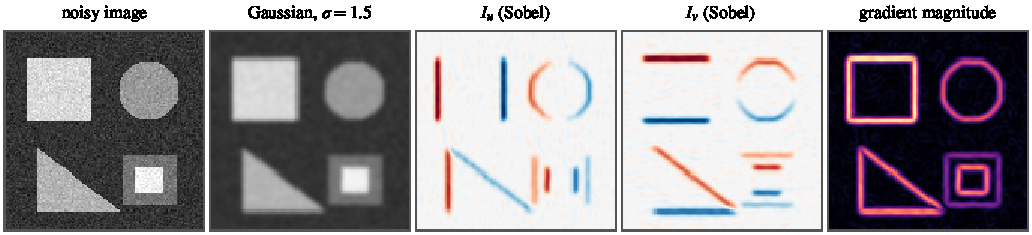
\includegraphics[width=\textwidth]{fig_image_filters.pdf}
  \caption{A synthetic noisy image, its Gaussian smoothing ($\sigma = 1.5$~px), its Sobel derivatives $I_u$ and $I_v$, and the gradient magnitude. Vertical edges respond in
  $I_u$, horizontal edges in $I_v$; corners respond in both, which is what corner detectors look for.}
  \label{fig:image-filters}
\end{figure}

% ==============================================================================
\section{Sampling, aliasing and pyramids}
\label{sec:pyramids}

\subsection{Aliasing in images}

An image is a sampled signal, and the sampling theorem (\cref{ch:processes}) applies in each direction: a pixel grid can represent spatial frequencies up to half a
cycle per pixel. Shrinking an image by keeping every other pixel halves the representable frequency. Any finer detail does not vanish: it \emph{aliases} into false
coarse patterns (moir\'e). The cure is the same as for any sampled signal: low-pass filter, by blurring, before down-sampling.

\begin{figure}[t]
  \centering
  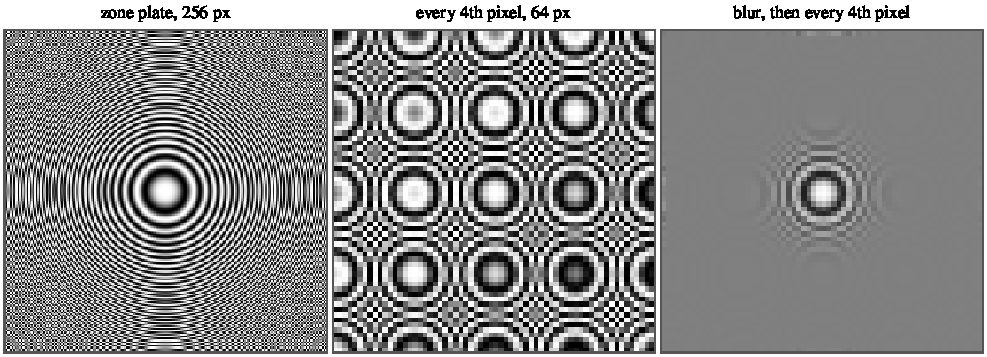
\includegraphics[width=\textwidth]{fig_aliasing_image.pdf}
  \caption{Aliasing in images. A ``zone plate'', whose spatial frequency increases away from the center (left), is shrunk four times by keeping every fourth pixel
  (middle) and by Gaussian blurring first (right). Naive sub-sampling creates false ring patterns; blurring removes the frequencies that cannot be represented.}
  \label{fig:aliasing-image}
\end{figure}

\subsection{Gaussian pyramids}

\index{image pyramid}
A \term{Gaussian pyramid} is a sequence of images, each a blurred and half-resolution copy of the previous one:
\begin{equation}
  I_{\ell+1} = \downarrow_2\big(G * I_\ell\big),
\end{equation}
where $G$ is a small Gaussian (OpenCV's \code{pyrDown} uses the binomial kernel $\tfrac1{16}[1, 4, 6, 4, 1]$ in each direction) and $\downarrow_2$ keeps every second row and
column. Level $\ell$ has $2^{-\ell}$ of the original resolution in each direction, so a pixel position $u_0$ at level 0 corresponds to $u_\ell \approx u_0/2^\ell$ at level $\ell$ (up
to half-pixel conventions). The whole pyramid costs only a third more memory than the original image ($1 + \tfrac14 + \tfrac1{16} + \cdots = \tfrac43$).

\begin{figure}[t]
  \centering
  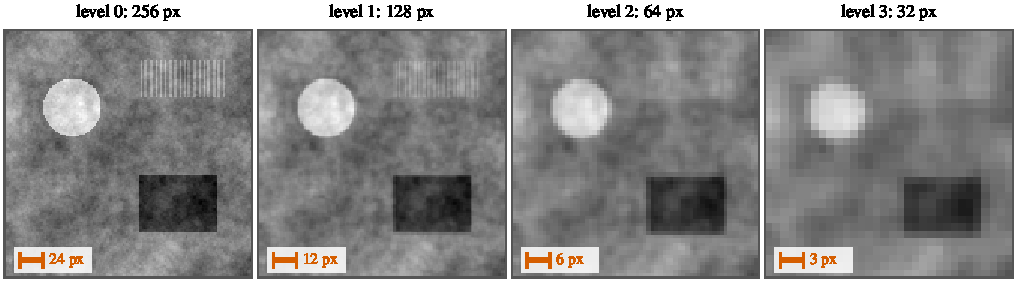
\includegraphics[width=\textwidth]{fig_pyramid.pdf}
  \caption{Four levels of a Gaussian pyramid of a textured synthetic image, displayed at a common size. Fine texture disappears level by level; coarse structure
  survives. A displacement of 24~px at level 0 is a displacement of 3~px at level 3.}
  \label{fig:pyramid-levels}
\end{figure}

Pyramids serve two purposes in the front end. Motion that is large in pixels at full resolution is small at coarse levels, where an iterative tracker can
capture it (\cref{ch:frontend}). And structures of different sizes are best detected at different scales.

% ==============================================================================
\section{Interpolation}
\label{sec:interpolation}

\index{bilinear interpolation}
Sub-pixel tracking needs image values and gradients at non-integer positions. Writing a position as $(u_0 + a, v_0 + b)$ with integer $(u_0, v_0)$ and fractional parts
$a, b \in [0, 1)$:
\begin{itemize}
  \item \emph{nearest neighbor} takes the closest pixel: fast, but the result jumps as the position moves, which ruins sub-pixel accuracy;
  \item \term{bilinear interpolation} interpolates linearly in $u$ along the two neighboring rows and then linearly in $v$ between the results:
  \begin{equation}
    I(u_0 + a, v_0 + b) = (1 - a)(1 - b)\,I_{00} + a(1 - b)\,I_{10} + (1 - a)b\,I_{01} + ab\,I_{11},
  \end{equation}
  with $I_{ij} = I[u_0 + i, v_0 + j]$. The result is continuous, and the weights are the areas of the rectangles opposite each corner;
  \item \emph{bicubic} interpolation fits a smooth cubic patch to a $4\times4$ neighborhood; it has continuous derivatives at the cost of 16 pixels per sample.
\end{itemize}
Lucas--Kanade trackers use bilinear interpolation for both the image and its gradients. With images represented as 8-bit integers, implementations use fixed-point
weights for speed, which limits the attainable sub-pixel resolution to a few hundredths of a pixel, well below the noise of real tracking.

% ==============================================================================
\section{Finding local maxima}

Detectors compute a response map (corner strength, for example) and select the pixels where it is large \emph{and} locally maximal. \termi{Non-maximum suppression}{non-maximum suppression}
keeps a pixel only if its response exceeds a threshold and is the largest in its neighborhood (a $3\times3$ window, or a larger radius to enforce spacing between
detections). The location of a maximum can then be refined below the pixel grid by fitting a parabola through the response $r_{-1}, r_0, r_1$ at the maximum and its two
neighbors in each direction; the vertex lies at the offset
\begin{equation}
  \delta = \frac{r_{-1} - r_{1}}{2\,(r_{-1} - 2r_0 + r_{1})}
\end{equation}
pixels from the center. Sub-pixel accuracy at the detection stage is less important for tracking-based front ends, whose tracker refines positions anyway.

% ==============================================================================
\section{Photometric changes}

Intensity-based methods assume that a scene point keeps its brightness between frames (\cref{ch:frontend}). Auto-exposure, lighting changes and non-Lambertian
surfaces violate this. A common model is an affine change, $I_2 \approx \alpha I_1 + \beta$. Gradients are unaffected by $\beta$, and comparing patches after subtracting their
means and dividing by their standard deviations (\emph{zero-mean normalized cross-correlation}) is unaffected by both. Some trackers estimate $\alpha$ and $\beta$
along with the motion; others pre-process images, for example with histogram equalization, to reduce the variation.

\begin{takeaways}
\begin{itemize}
  \item Filtering is convolution with a kernel; separable kernels cost $2k$ instead of $k^2$ per pixel.
  \item Gaussian smoothing reduces noise without ringing; variances of cascaded Gaussians add.
  \item Derivatives amplify noise; Sobel, Scharr and derivative-of-Gaussian kernels smooth and differentiate at once.
  \item Down-sampling without blurring aliases; a Gaussian pyramid blurs and halves the resolution at each level.
  \item Bilinear interpolation gives continuous sub-pixel samples; non-maximum suppression and parabola fits localize detections.
  \item Normalize patches when brightness may change between frames.
\end{itemize}
\end{takeaways}

\begin{exercises}
  \item Show that the 2D Gaussian kernel is separable, and that filtering with it costs $2k$ operations per pixel for a $k$-tap kernel.
  \item Show that convolving $\tfrac12[1, 1]$ with itself repeatedly produces the binomial kernels, and that their variance grows linearly with the number of
        convolutions.
  \item Compute the response of the Sobel kernel $S_u$ to a linear ramp $I(u, v) = cu$, and explain the factor 8.
  \item Generate a zone plate and reproduce \cref{fig:aliasing-image}. How large must the blur be before shrinking by 4?
  \item Derive the bilinear interpolation formula by interpolating first along $u$ and then along $v$, and show that the result does not depend on the order.
  \item Derive the parabola-vertex formula for sub-pixel peak refinement.
\end{exercises}
% Solutions to the exercises of Chapter 21.
\begin{solutions}
  \item The exponent splits, $e^{-(u^2 + v^2)/2\sigma^2} = e^{-u^2/2\sigma^2}e^{-v^2/2\sigma^2}$, and so does the constant, $\frac1{2\pi\sigma^2} = \frac1{\sqrt{2\pi}\sigma}\cdot\frac1{\sqrt{2\pi}\sigma}$, so
        $G_\sigma(u, v) = g_\sigma(u)g_\sigma(v)$. Sampled on a square $k\times k$ grid the kernel is the outer product $h = gg\T$ of the sampled 1D kernel, and normalizing
        each 1D kernel to unit sum normalizes the product too. Then
        \[
          (h * I)[u, v] = \sum_jg[j]\Big(\sum_ig[i]\,I[u - i, v - j]\Big):
        \]
        the inner sum filters every row with $g$ ($k$ multiplications per pixel) and the outer sum filters the columns of the result ($k$ more), $2k$ in total
        instead of $k^2$. For $\sigma = 1.5$ truncated at $\pm3\sigma$ ($k = 11$) this is 22 instead of 121. Truncating to a \emph{disk} instead of a square would destroy
        the factorization.

  \item The kernel $[a_0, \dots, a_n]$ corresponds to the polynomial $\sum_ia_iz^i$, and convolution of kernels is multiplication of polynomials. Convolving
        $\tfrac12[1, 1]$ with itself $n$ times gives $\big(\tfrac12(1 + z)\big)^n = 2^{-n}\sum_i\binom{n}{i}z^i$: the binomial kernels $\tfrac14[1, 2, 1]$, $\tfrac18[1, 3, 3, 1]$, $\tfrac1{16}[1, 4, 6, 4, 1]$, \dots.
        A non-negative kernel with unit sum is a probability distribution, and the convolution of two distributions is the distribution of the sum of
        independent variables, whose variances add (\cref{ch:prob}). The two-point kernel $\tfrac12[1, 1]$ has variance $\tfrac14$, so the $n$-fold kernel has variance $n/4$:
        $\tfrac12$ for $[1, 2, 1]$, $1$ for $[1, 4, 6, 4, 1]$. By the central limit theorem the binomial kernels approach Gaussians with $\sigma = \sqrt n/2$; OpenCV's
        \code{pyrDown} kernel is a Gaussian with $\sigma = 1$~px.

  \item At pixel $(u, v)$ the correlation sums $S_u[j, i]\,c\,(u + i)$. In each row the weights $-1, 0, 1$ give $c(u + 1) - c(u - 1) = 2c$, and the three rows are
        weighted $1, 2, 1$, so
        \[
          (S_u\star I)[u, v] = (1 + 2 + 1)\cdot2c = 8c,
        \]
        everywhere, for a true derivative $I_u = c$. The factor 8 is the product of the smoothing kernel's sum (4) and the distance between the differenced
        pixels (2). Divide by 8 to obtain the gradient (by 32 for Scharr, whose smoothing kernel sums to 16). With convolution instead of correlation the
        kernel is flipped and the response is $-8c$: check the sign convention of whatever library you use.

  \item A zone plate $I = \tfrac12 + \tfrac12\cos(\pi r^2/n)$ on an $n\times n$ grid (the figure uses $n = 256$) has phase $\pi r^2/n$, hence local frequency $r/n$ cycles per pixel. After
        keeping every fourth pixel the representable limit is $\tfrac18$ cycle per original pixel, so the true rings beyond $r = n/8 = 32$ cannot be represented
        and should become uniform gray; instead, naive sub-sampling folds them into false rings, with new ``centers'' where the frequency is a multiple of the
        new sampling rate $\tfrac14$. A Gaussian blur multiplies frequency $f$ by $e^{-2\pi^2\sigma^2f^2}$. Measuring the false pattern in the region $48 < r < 128$:
        \begin{center}\small
        \begin{tabular}{@{}l c c c c c@{}}
        \toprule
        blur $\sigma$ (px) & 0 & 1 & 1.5 & 2 & 3 \\
        \midrule
        RMS of false pattern & 0.353 & 0.061 & 0.018 & 0.005 & 0.002 \\
        response at $f = \tfrac18$ (kept detail) & 1 & 0.73 & 0.50 & 0.29 & 0.06 \\
        response at $f = \tfrac14$ (aliases to DC) & 1 & 0.29 & 0.06 & 0.007 & $10^{-5}$ \\
        \bottomrule
        \end{tabular}
        \end{center}
        A blur of $\sigma \approx 2$~px, half the shrink factor, removes the aliasing (as in \cref{fig:aliasing-image}); much more also removes detail the smaller image could
        have kept. The same rule, $\sigma \approx s/2$ for a shrink by $s$, gives \code{pyrDown}'s $\sigma = 1$ for $s = 2$.

  \item Along the row $v_0$, linear interpolation gives $(1 - a)I_{00} + aI_{10}$, and along the row $v_0 + 1$, $(1 - a)I_{01} + aI_{11}$. Interpolating these linearly in $v$ with
        weights $1 - b$ and $b$ gives the formula of \cref{sec:interpolation}. In the other order, the columns give $(1 - b)I_{00} + bI_{01}$ and $(1 - b)I_{10} + bI_{11}$, and
        interpolating in $u$ gives $(1 - a)(1 - b)I_{00} + (1 - a)bI_{01} + a(1 - b)I_{10} + abI_{11}$, the same four products. Without expanding: both results have the form
        $c_0 + c_1a + c_2b + c_3ab$ and take the four corner values at the corners, and those four conditions determine the four coefficients uniquely. The
        interpolant is linear along every row and column but quadratic along diagonals, and its derivatives jump at pixel boundaries.

  \item Fit $r(x) = Ax^2 + Bx + C$ through $(-1, r_{-1})$, $(0, r_0)$, $(1, r_1)$: $C = r_0$, $A + B + C = r_1$ and $A - B + C = r_{-1}$, so
        $B = \tfrac12(r_1 - r_{-1})$ and $A = \tfrac12(r_{-1} - 2r_0 + r_1)$. The vertex is at
        \[
          \delta = -\frac{B}{2A} = \frac{r_{-1} - r_1}{2(r_{-1} - 2r_0 + r_1)} .
        \]
        If $r_0$ is the largest of the three, $A < 0$ (a maximum), and $|r_{-1} - r_1| \le (r_0 - r_{-1}) + (r_0 - r_1) = 2|A|$, so $|\delta| \le \tfrac12$: the refined peak stays within
        the pixel. Real peaks are not parabolas, and the fit is biased toward the pixel center: for a Gaussian peak of width $\sigma = 1$~px at a true
        offset of $0.3$~px it returns $0.25$, a bias of up to $0.05$~px, larger for sharper peaks.
\end{solutions}

